\chapter{TikZ gyorstalpal\'o}

\section{Alapok}

A \verb|\usepackage{tikzpicture}| kell a library implementálásához A \verb|\begin{tikzpicture}| és \verb|\end{tikzpicture}| parancsok közé kell helyezni a rajzolandó ábrát. A TikZ úgy működik, mint egy rajztábla. Egyesével kell az objektumokat rárajzolni, esetenként egy ciklusban többet is lehet egyszerre (lásd lejjebb). \textbf{Minden parancsot egy  ;-vel kell lezárni.}

A \verb|\begin{tikzpicture}["paraméterek"]| ebben a szögletes zárójelben kell megadni a rajztábla paramétereit. Ilyenek:
\begin{itemize}
    \item "\texttt{scale = 3}"  -- a képet nyújtja, kivéve a betű méretet
    \item "\texttt{xscale = 4, yscale = 5}"  -- ugyanez, csak merőlegesen affin képet ad
\end{itemize}

A rajzolásra két különböző, de általában mindenre elég parancs a \verb|\draw| és \verb|\filldraw| . A sima rajzolás csak körvonalat rajzol, a másik pedig automatikusan ugyanazzal a színnel kitölti az alakzatot. Mindkettő parancsnak meg kell mondani, hogy:

\begin{itemize}
    \item Hova: \texttt{(x, y)}, \texttt{(fok:hossz)}
    \item Mit: \texttt{node}, \texttt{--} (edge), \texttt{circle}, \texttt{rectangle}, \texttt{arc}
    \item Stílusban: \texttt{[color, ultra thin, fill]} -- ez lehet üres, ilyenkor a rajztábla stílusát használja
\end{itemize}

A node-ok kicsit trükkösebbek, róluk a gráfok részben lehet részletesebben olvasni.

%\begin{minted}{tex}
\begin{Example}
\begin{tikzpicture}[scale=3]
    %a köröknek a kp.-át és sugarát kell megadni
    \draw (0,0) circle (0.4 cm) [color = blue!90];
    \filldraw (1,0) circle (0.4 cm) [color = red!90];
    
    %a téglalapoknak a balalsó és jobbfelső csúcsait kell megadni
    \draw (2-0.4, -.4) rectangle (2+0.4, .4) [ultra thick, fill=black!20];
    
    %a törött vonalakat csúcsról csúcsra kell megadni
    \draw  (3-0.3, -0.3) -- (3-0.3, 0.4) -- (3+0.4, -0.4) -- (3+0.4, 0.4);
    
    %ami sokkal menőbb, például egy rácsbejáráshoz az íveltvonalak
    \draw[thick,rounded corners=8pt, color=pink!200] (4-0.3, -0.3) -- (4-0.3, 0.4) 
    -- (4+0.4, -0.4) -- (4+0.4, 0.4);
    
    %Ha a törött vonalat lezárnád érdemes a --cycle befejezést írni a kezdő csúcs 
    %megismétlése helyett.
\end{tikzpicture}
\end{Example}
%\end{minted}


\subsection{Illesztés}

Az első fejezetben leírtakat érdemes alkalmazni. A \texttt{\bs clip} parancsot érdemes használni. Nem csak arra jó, hogy kivágjuk a kép egy részét, de beállítja a kép keretét, ha azzal kezdjük. Erre persze lehet használni a \verb|\useasboundingbox| parancsot amivel megadhatunk például egy téglalappal határolt fix keretét a képnek. Amit ezen kívül rajzoltál nem fogja megjeleníteni.

\begin{Example}
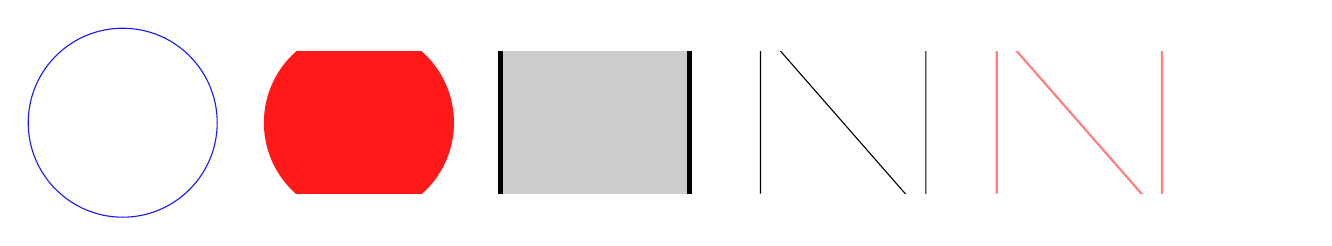
\begin{tikzpicture}[scale=3]        
    \draw (0,0) circle (0.4 cm) [color = blue!90];
    %Itt vágunk ami azt okozza, hogy az előző kör nem sérült
    \clip (-0.3, -0.3) rectangle (5, 0.3);
    \filldraw (1,0) circle (0.4 cm) [color = red!90];
    \draw (2-0.4, -.4) rectangle (2+0.4, .4) [ultra thick, fill=black!20];
    %Lehet relatív megadni a távolságokat, hogy ne kelljen mindent papíron kiszámolni
    %Ha csak sima +-t használsz, akkor a kezdő csúcstól viszonyít
    \draw  (3-0.3, -0.3) -- ++(0, 0.7) -- ++(0.7, -0.8) -- ++(0, 0.8);
    \draw[thick,rounded corners=8pt, color=pink!200]     (4-0.3, -0.3) -- (4-0.3, 0.4) -- (4+0.4, -0.4) -- (4+0.4, 0.4);
\end{tikzpicture}
\end{Example}

\subsection{Színek, egyebek}

Be lehet állítani vonalvastagságot, színt és még színátmenetes ábrát is egyszerű csinálni.
\begin{itemize}
    \item Vastagságok: \{\verb|ultra|, \verb|very|, \} + \{\verb|thin|, \verb|thick|\}
    \item Színek: \{ \verb|red|, \verb|green|, \verb|blue|, \verb|cyan|, \verb|magenta|, \verb|yellow|, \verb|black|, \verb|gray|, \verb|darkgray|, \verb|lightgray|, \verb|brown|, \verb|lime|, \verb|olive|, \verb|orange|, \verb|pink|, \verb|purple|, \verb|teal|, \verb|violet|, \verb|white| \}
    \item Vonal típusok: \{\verb|dashed|, \verb|dotted|\}
    \item Vonal összekötési lehetőségek (advanced): \begin{itemize}
        \item \verb|line cap = {round, rect, butt}|
        \item \verb|rounded corners = 5mm|
        \item \verb|line join = {round, bevel, mitern}|
        \end{itemize}
\end{itemize}

\begin{Example}
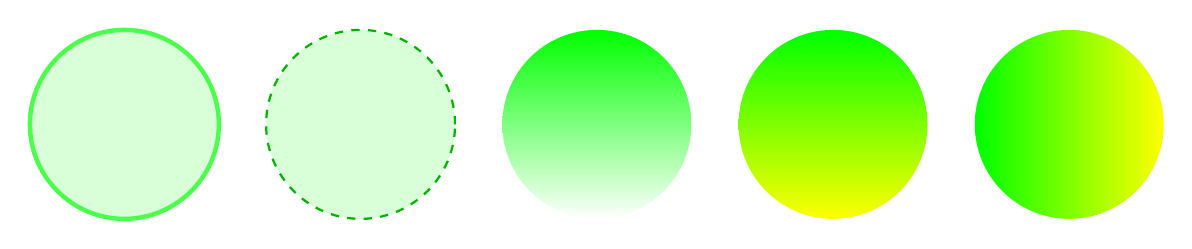
\begin{tikzpicture}[scale=3]
    \draw (0,0) circle (0.4) [color = green!70, fill = green!15, ultra thick];
    \draw (1,0) circle (0.4)     [color = green!70!black, fill = green!15, thick, dashed];
    \shade (2,0) circle (0.4) [top color = green];
    \shade (3,0) circle (0.4) [top color = green, bottom color = yellow];
    \shade (4,0) circle (0.4) [left color = green, right color = yellow];
\end{tikzpicture}
\end{Example}

\section{Sokszögek rajzolása, for ciklusok}

Az, hogy lehet for ciklusokat írni, nagyban segít a valamilyen szempontból szimmetrikus ábrák elkészítésében. A for ciklusok hasonlóan más nyelvekhez bevezetnek egy változót, ami végig fut adott értékeken és végrehajtja a megadott parancsokat egyesével (jobb ha nem számít a sorrend).  Lehet egymásba ágyazott ciklusokat írni, de lehet párhuzamosan két vagy több változót egyszerre változtatni. Például \verb|\foreach \x in {1,2,3,4}{<commands>}| Ennél lehet komolyabb dolgokat is csinálni, lásd a példákat.

Eddig nem volt róla szó, de a hagyományos koordinátázás helyett lehet polárkoordinátákat is használni. \verb|(90:1cm)| -- 90 fok, 1 cm messze

A képet lehet transzformálni erre pár példa: \verb|xshift|, \verb|yshift|, \verb|rotate|

\begin{Example}
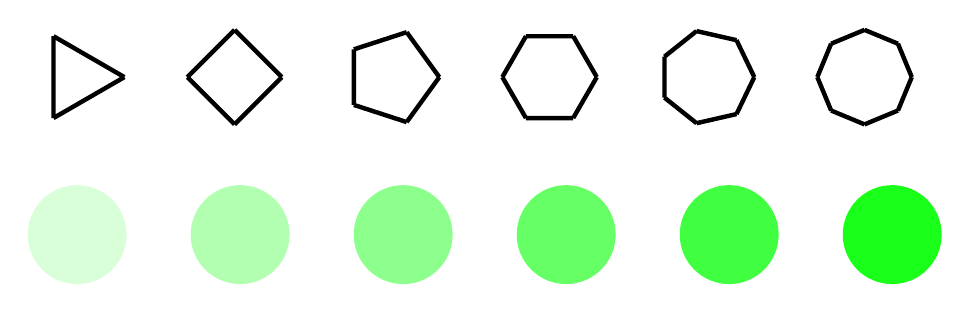
\begin{tikzpicture}[scale = 2, ultra thick]
    \foreach \n in {3, ..., 8}{    \draw (\n-3,0) \foreach \d in {1, ..., \n}{ %MAGIC DANGER        
            +(\d*360/\n:0.3cm) -- +(\d*360/\n + 360/\n:0.3cm)    }; 
            %Az, hogy ilyet lehet csinálni szerintem egyszerre undorító és hasznos
            %Ez kell ahhoz, hogy a szín mögé lehessen írni változót (nem igazán lehet képletet)
            \pgfmathsetmacro\i{\n*15-30} 
            \filldraw [xshift = \n-3, color = green!\i] (\n-3,-1) circle (0.3cm);
    }
\end{tikzpicture}
\end{Example}

\section{Rácsok, szöveg beillesztése}

A \verb|\draw grid| parancsot lehet négyzetrács készítésre használni a \verb|\foreach| helyett. Meg kell adni a lépésközt és egy téglalapot ami határolja.

Szöveget beilleszteni úgy kell, hogy egy Node-ot töltünk fel szöveggel. Paraméterként meg lehet adni, hogy az adott pozícióhoz képest, hol helyezkedjen el a csúcs és így a szöveg, ezt az \verb|anchor=<direction>| paraméterrel lehet megadni. A \verb|fill=white| paraméter megadásával az is elérhető, hogy a szöveg/szám alatt megszakadjanak a vonalak, így egy sokkal esztétikusabb végeredményt kapunk. 

Itt különösen kiemelném a \verb|\clip| parancs fontosságát. Ha egy ábrát szeretnék nagyban és kicsiben is használni elég megismételni a kódot és megadunk egy keretet, ahol kíváncsiak vagyunk az ábra részleteire. 

\begin{Example}
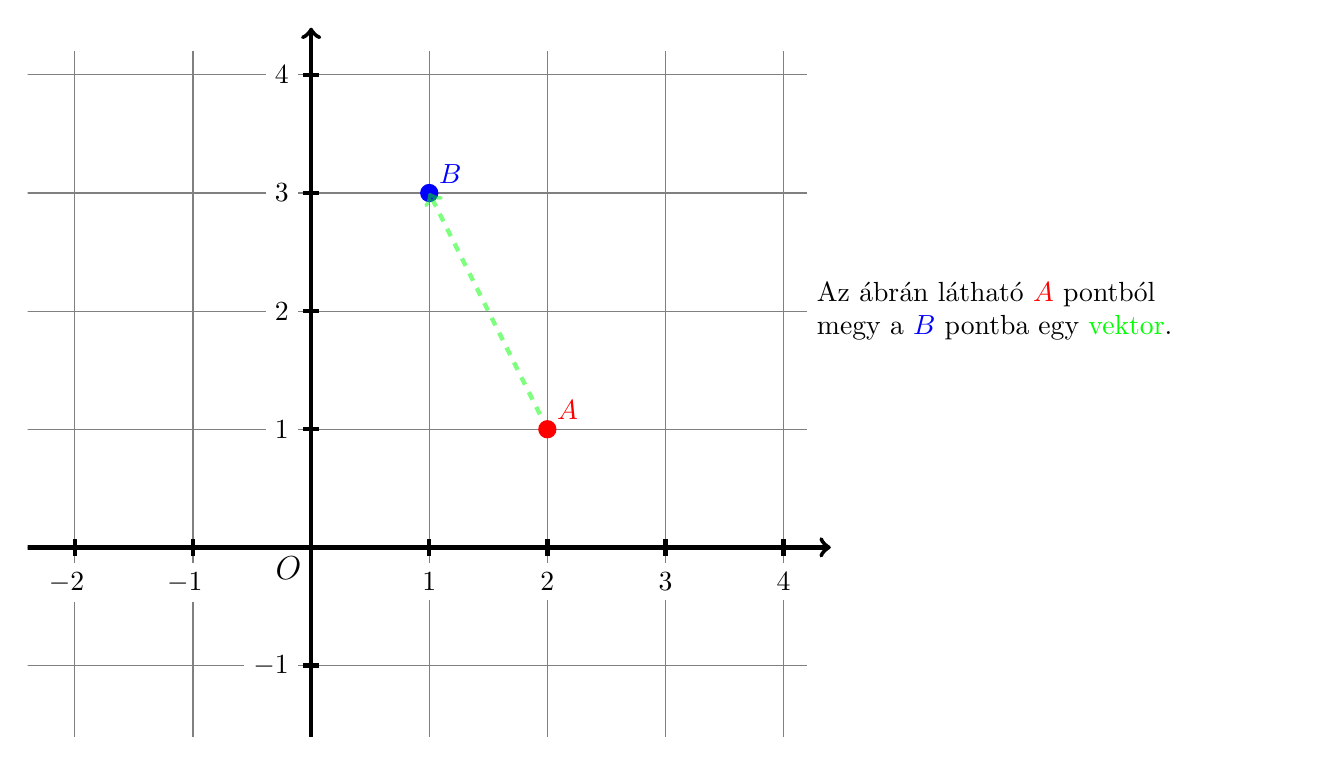
\begin{tikzpicture}[scale = 3]
	\clip (-1.2, -0.8) rectangle (4.2,2.2); %Ez csak azért, hogy jobban ráférjen a honlapra
	%grid
	\draw[step = 0.5, color=gray] (-2.1,-2.1) grid (2.1,2.1);
	%axes
	\draw[->, ultra thick] (0,-2.2) -- (0,2.2);
	\draw[->, ultra thick] (-2.2,0) -- (2.2,0);
	%texts
	\draw (0,0) [fill = white, anchor = north east] node {\large $O$};
	
	%y-tengely
	\foreach \label in {1, 2, 3, 4}
	\pgfmathsetmacro\pos{\label/2}
	\draw [ultra thick](-1pt,\pos) -- (1pt, \pos) node [fill = white, left, xshift = -7pt] {$\label$};
	\foreach \label in {-1, -2, -3, -4}
	\pgfmathsetmacro\pos{\label/2}
	\draw [ultra thick](-1pt,\pos) -- (1pt, \pos) node [fill = white, left, xshift = -7pt] {$\label$};
	
	%x-tengely		
	\foreach \label in {1, 2, 3, 4}
	\pgfmathsetmacro\pos{\label/2}
	\draw [ultra thick](\pos, 1pt) -- (\pos, -1pt) node [fill = white, below, yshift = -2pt] {$\label$};
	\foreach \label in {-1, -2, -3, -4}
	\pgfmathsetmacro\pos{\label/2}
	\draw [ultra thick](\pos, 1pt) -- (\pos, -1pt) node [fill = white, below, yshift = -2pt, xshift = -3pt] {$\label$};
	
	%ábra
	\draw (1, 0.5) node [color=red, anchor = south west] {$A$};
	\draw (0.5, 1.5) node [color=blue, anchor = south west] {$B$};
	\draw (0.5,1.5) node [color=blue, circle, fill=blue, scale =0.7] {};
	\draw [->, green, dashed, ultra thick, opacity=0.5] (1, 0.5) -- (0.5, 1.5);
	\draw (1, 0.5) node [color=red, circle, fill=red, scale =0.7] {};
	\draw[xshift=2.1cm, yshift=1cm] node[right,text width=5cm]
	{Az ábrán látható {\color{red} $A$} pontból megy a {\color{blue} $B$} pontba egy {\color{green} vektor}.};
\end{tikzpicture}
\end{Example}

\section{Gráfok}

Lehet gráfokat úgy definiálni, hogy a csúcsokat megadjuk és utána az élek már a meglévő objektumainkat (csúcsok) kössék össze. Ez azért hasznos, mert rugalmasabb lesz az ábra. Ha esetleg változtatnánk a gráfon egy új csúcs behozásával nem kell az egész ábrát koordinátánként átírni. Elég csak a csúcsokat áthelyezni, a többit a TikZ megcsinálja nekünk. Ami még különösen hasznos, hogy tudunk a programban a csúcsoknak nevet adni és utána ezt a nevet használni referenciaként, hogy egy sokkal átláthatóbb kódot kapjunk végeredményül. Ez nem összekeverendő a csúcshoz tartozó szöveggel.

Amit szintén itt mutatnék be az a dinamikus stílus kezelés. Lehet ugyanis általunk előre definiált stílusokat megadni, hogy utána csak elég legyen annyit írni, hogy \verb|[fontos]| vagy \verb|[seged]|. Ezzel is azt érjük el, hogy olvashatóbb és egységesen változtathatóbb lesz a kód és így az ábránk.

A csúcsok és élek szövegezésére is sok lehetőséget ad a TikZ. A \verb|label=<direction>:<text>| paraméter, akár többszöri használatával tudunk mindenféle szöveggel/névvel ellátni az ábránkat.

Lehet az éleket hajlítani, kígyósítani és egyéb stilisztikai trükköket alkalmazni. Erre azt ajánlom, hogy a dokumentációt érdemes olvasgatni. A következő részben írok a görbe vonalakról, ott érdemes erről olvasni.

\begin{Example}
\usetikzlibrary{positioning,backgrounds}
\begin{tikzpicture}[auto, node distance = 1cm and 2cm]
	\tikzstyle{StartEnd}=[rectangle,draw=blue!50, fill=blue!20,thick, 			inner sep=0pt,minimum size=6mm]
	\tikzstyle{alayer}=[circle,draw=red!80,fill=red!20,thick, inner sep=0pt,minimum size=6mm]
	\tikzstyle{blayer}=[circle,draw=red!80,fill=red!40,thick, inner sep=0pt,minimum size=6mm]
	\tikzstyle{se-edge}=[->,very thick, color=blue!30]
	\tikzstyle{in-edge}=[->,very thick, color=red!30]
	
	%Nodes
	\node[StartEnd] (Start) [label = 135:\color{blue}\Large$S$] {};
	
	\node[alayer] (a3) [right = of Start, label=above:$a3$] {};
	\node[alayer] (a2) [above = of a3, label=above:$a2$] {};
	\node[alayer] (a1) [above = of a2, label=above:$a1$] {};
	\node[alayer] (a4) [below = of a3, label=above:$a4$] {};
	\node[alayer] (a5) [below = of a4, label=above:$a5$] {};
	
	\node[blayer] (b3) [right = of a3, label=above:$b3$] {};
	\node[blayer] (b2) [above = of b3, label=above:$b2$] {};
	\node[blayer] (b1) [above = of b2, label=above:$b1$] {};
	\node[blayer] (b4) [below = of b3, label=above:$b4$] {};
	\node[blayer] (b5) [below = of b4, label=above:$b5$] {};
	
	\node[StartEnd] (End)[right = of b3,label=45:\color{blue}\Large$C$] {};
	
	%Edges
	\draw[se-edge] (Start) to [out=45, in=180] (a1);
	\draw[se-edge] (Start) to [out=22.5, in=180] (a2);
	\draw[se-edge] (Start) to [out=0, in=180] (a3);
	\draw[se-edge] (Start) to [out=360-22.5, in=180] (a4);
	\draw[se-edge] (Start) to [out=360-45, in=180] (a5);
	
	\draw[se-edge] (b1) to [out=0, in=180-45] (End);
	\draw[se-edge] (b2) to [out=0, in=180-22.5] (End);
	\draw[se-edge] (b3) to [out=0, in=180] (End);
	\draw[se-edge] (b4) to [out=0, in=180+22.5] (End);
	\draw[se-edge] (b5) to [out=0, in=180+45] (End);
	
	\draw[in-edge] (a1) to (b2);
	\draw[in-edge] (a2) to (b1);
	\draw[in-edge] (a2) to (b5);
	\draw[in-edge] (a3) to (b5);
	\draw[in-edge] (a4) to (b1);
	\draw[in-edge] (a5) to (b3);
	\draw[in-edge] (a5) to (b5);
	
	%Layers
	\begin{pgfonlayer}{background}
		\filldraw [fill=black!20, draw=black] (a5.south -| a5.west) rectangle (a1.north -| a1.east);
		\filldraw [fill=black!20, draw=black] (b5.south -| b5.west) rectangle (b1.north -| b1.east);
	\end{pgfonlayer}
	
\end{tikzpicture}
\end{Example}

